\section{Introducción}

\begin{frame}{Desarrollo de aplicaciones con Microprocesadores}
    \begin{itemize}
        \item Aplicaciones sencillas (fácil implementarlas mediante un bucle while, algunos timers y algunas interrupciones)
Si la complejidad de la aplicación crece, el número de temporizaciones aumenta frente al número de timers disponibles en el microprocesador y la lógica de la misma es compleja, la gestión, desarrollo y depuración de la aplicación se complican enormemente.
        \item Para simplificar esta situación se han desarrollado Sistemas Operativos “ligeros” para ser implementados en arquitecturas basadas en microprocesadores. Su utilización permite que el desarrollo de software sea más sencillo, seguro, y eficiente, redundando en un mantenimiento más sencillo del software.      
    \end{itemize}
     \centering

\end{frame}

\begin{frame}{CMSIS-RTOS}
    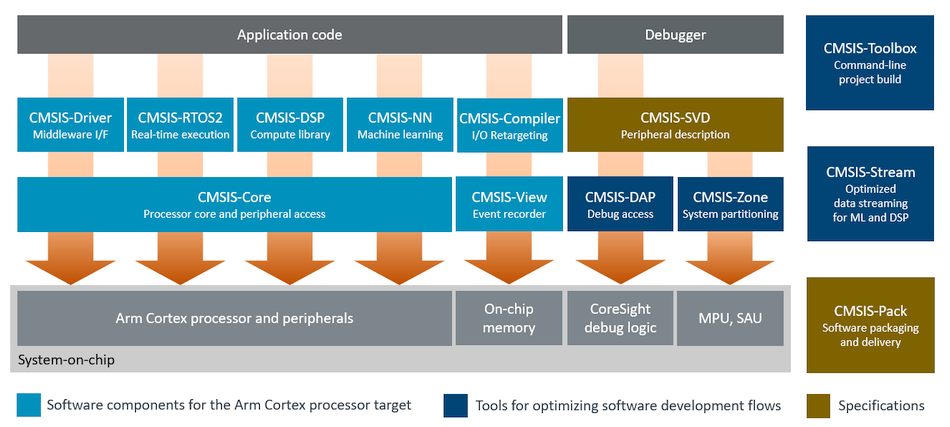
\includegraphics[scale=0.35]{presentation/cmsis_components.png}
\end{frame}

\begin{frame}{CMSIS-RTOS}
    \begin{itemize}
      \item API C/C++ para sistemas operativos en tiempo real
      \item Diseñado para procesadores Cortex M
      \item Versión a utilizar CMSIS-RTOS2. Está se puede configurar para usar los kernels CMSIS-RTX (o keil RTX5), freeRTOS, Zephyr, embOS, Azure Thread y Micrium.
      \item En SBM se usa 2.1.3 que se basa en CMSIS v5 con RTX \href{https://arm-software.github.io/CMSIS_5/RTOS2/html/index.html}{(Documentación 2.1.3)}
      \item ARM ya ha lanzado la versión 2.3.0 que se basa en CMSIS V6 \href{https://arm-software.github.io/CMSIS_6/latest/RTOS2/index.html}{(Documentación 2.3.0)}
    \end{itemize}
    
\end{frame}

\section{CMSIS-RTOS:Características}
\begin{frame}{CMSIS-RTOS: Características}
    \begin{itemize}
  \item \textbf{Aplicaciones multihilo}: basada en la utilización de hilos concurrentes.
  \item Aporta mecanismos de comunicación y sincronización entre hilos.
  \item \textbf{Thread}:
    \begin{itemize}
        \item Porción de código que realiza una función concreta.
        \item Típicamente es una función con un bucle infinito y sin retorno.
        \item El RTOS permite compartir la ejecución con otros threads.
        \item 5 estados: \texttt{Running}, \texttt{Ready}, \texttt{Waiting/Blocked}, \texttt{Inactive}, \texttt{Terminated}.
    \end{itemize}
  \item \textbf{Scheduler}:
    \begin{itemize}
        \item Planificación y compartición de los recursos de CPU.
        \item Gestiona la ejecución de threads asignando tiempo (\texttt{SysTick}) de procesador a cada hilo.
    \end{itemize}
  \item \textbf{Timeslice}:
    \begin{itemize}
        \item Período de tiempo asignado a cada hilo.
        \item Múltiplo del Tick (5 por defecto) generado por el \texttt{SysTick} (1ms por defecto).
    \end{itemize}
\end{itemize}

\end{frame}

\begin{frame}{CMSIS-RTOS: Planificador}
    \begin{itemize}
      \item \textbf{Pre-emptive}
          \begin{itemize}
            \item Desalojo de hilos “ menos prioritarios” por hilos “ mas prioritarios”.
          \end{itemize}
      \item \textbf{Round-Robin}
          \begin{itemize}
            \item Todos los hilos con la misma prioridad.
            \item Se ejecutan unos detrás de otros en secuencia durante un “timeslice”.
      \end{itemize}
      \item \textbf{Round-Robin Pre-emptive}
          \begin{itemize}
            \item Los hilos pueden tener distinta prioridad.
            \item Los hilos con igual prioridad se ejecutan de forma Round-Robin mientras no haya otro hilo de +prioridad en estado \texttt{READY}.
            \item Cuidado con las prioridades para no “colgar” la aplicación.
            \item Por defecto en CMSIS-RTOS - RTX.
      \end{itemize}
      \item \textbf{Cooperative Multitasking}
          \begin{itemize}
            \item Todos los hilos con igual prioridad.
            \item No Round-Robin.
            \item Cada hilo se ejecuta hasta bloquearse (pasa a \texttt{WAIT}) o hasta pasar la ejecución a otro (\texttt{yield}).
          \end{itemize}
    \end{itemize}
\end{frame}


\begin{frame}[fragile]{CMSIS-RTOS: Estados en Threads}
    \begin{itemize}
        \item El planificador del SO es el encargado de gestionar la ejecución de un thread
        \item Estados de un thread:
       \begin{itemize}
          \item \textbf{RUNNING}: thread actualmente en ejecución.
          \item \textbf{READY}: threads preparados para ser ejecutados. Una vez que la tarea que se está ejecutando ha consumido su \textit{timeslice}, la siguiente tarea con máxima prioridad pasa a \textbf{RUNNING}.
          \item \textbf{BLOCKED/WAITING}: threads esperando la ocurrencia de algún evento.
          \item \textbf{TERMINATED}: threads terminados pero sin liberar recursos.
          \item \textbf{INACTIVE}: threads no creados o terminados. No consumen ningún recurso.
        \end{itemize}
    \end{itemize}
    
\end{frame}
\begin{frame}{Máquina de estados para un thread}
    \begin{center}    
        \resizebox{0.75\textwidth}{!}{
        \begin{tikzpicture}[shorten >=1pt, node distance=8cm, on grid, auto, font=\fontsize{18}{22}\selectfont, line width = 3pt]
          \node[state,  minimum size=3cm, fill=green] (ready) {ready};
          \node[state,  minimum size=3cm, fill=orange] (running) [right=of ready] {running};
          \node[state,  minimum size=3cm, fill=red] (blocked) [right=of running] {blocked};
          \node[state, minimum size=3cm] (inactive-terminated) [below=of running] {inactive-terminated};
        
          \path[->]
            (ready) edge  node {preempt} (running)
            (ready) edge  node {terminate} (inactive-terminated)
            (inactive-terminated) edge  node {create} (ready)
            (running) edge  node {preempt} (ready)
            (blocked) edge [bend left] node {events occur} (running)
            (running) edge [bend left] node {wait} (blocked)
            (blocked) edge [bend right] node {events occur} (ready)
            (blocked) edge [bend left] node {terminate} (inactive-terminated)
            (running) edge node {terminate} (inactive-terminated)
            (inactive-terminated) edge node {create} (running);
        \end{tikzpicture}
        }
    \end{center}
\end{frame}

\section{Código básico}
\begin{frame}[fragile]{Thread in Keil Microvision}
    \begin{minted}[fontsize=\scriptsize, bgcolor=blue!5]{c}
    #include "cmsis_os2.h"
    
    osThreadId_t tid_thread; // tid_thread identifica al thread.Se usará en funciones específicas del RTOS
    ...
    
    tid_Thread = osThreadNew(Thread, NULL, NULL);
    if (tid_Thread == NULL) {
        return(-1);
    }


    void Thread (void *argument){
        // inserte el código que solo quiera que se ejecute una vez
        while(1){
        // inserte el código que quiera que se ejecute continuamente
        
        }
        // nunca se llega a este punto en este ejemplo
    
    }
    \end{minted}
    \begin{itemize}
        \item Es altamente aconsejable crear un fichero de cabecera donde se deberán declarar la función de inicio para poder ser utilizados por otros módulos del software

    \end{itemize}
\end{frame}

\begin{frame}[fragile]{Implementación de aplicaciones con Threads}
    \begin{columns}
        \begin{column}{0.50\textwidth}
            \begin{minted}[fontsize=\scriptsize, bgcolor=blue!5]{c}
// Fichero con thread ThDisplay.c
#include "cmsis_os2.h"
#include "ThDisplay.h"

osThreadId_t tid_ThDisplay; 
...

tid_ThDisplay = osThreadNew(ThDisplay, 
                NULL, NULL);
if (tid_ThDisplay == NULL) {
    return(-1);
}


void ThDisplay (void *argument){
    int ciclo=0;
    Init_display();
    while(1){
    .....
    
    }
   

}
            \end{minted}
        \end{column}
    \begin{column}{0.50\textwidth}
        \begin{minted}[fontsize=\scriptsize, bgcolor=blue!5]{c}
        // Fichero main.c
        #include "ThDisplay.h"
        int main(void){
            int status=0;
            HAL_Init();
            SystemClock_Config();
            SystemCoreClockUpdate();
        #ifdef RTE_CMSIS_RTOS2
            oskernelInitilize();
            status|= Init_ThDisplay();
            osKernelStart();
        #endif
        }
        \end{minted}
        \begin{minted}[fontsize=\scriptsize, bgcolor=blue!5]{c}
        // Fichero de cabecera  ThDisplay.h    
        #include "stm32f4xx_hal.h"
        
        #ifndef __THDISPLAY__H
        #define __THDISPLAY__H
            #define S_PINTA  0x0001U
            int Init_ThDisplay(void);
        #endif
        
        \end{minted}
    \end{column}
    \end{columns}
    \begin{itemize}
        \item Es altamente aconsejable crear un fichero de cabecera donde se deberán declarar la función de inicio para poder ser utilizados por otros módulos del software

    \end{itemize}
\end{frame}

\section{Sincronización}
\begin{frame}{CMSIS RTOs Sincronización}
    \begin{columns}
        \begin{column}{0.50\textwidth}
            \begin{itemize}
                \item Una aplicación usará múltiples threads y recursos que hay que sincronizar
                \item ¿Cúal es el problema?
                    \begin{itemize}
                        \item Varios threads se ejecutan concurrentemente y quieren usar el mismo recurso compartido que puedes ser software o hardware
                        \item Hay que garantizar el uso secuencial del recurso compartido
                    \end{itemize}
                \item ¿Cuál es la solución?
                \begin{itemize}
                    \item Usar recursos como eventos, flags, colas, semáforos, etc
                    \item CMSIS-RTOS V2 implementa una API con estos recursos
                \end{itemize}
            \end{itemize}    
        \end{column}
        \begin{column}{0.50\textwidth}
            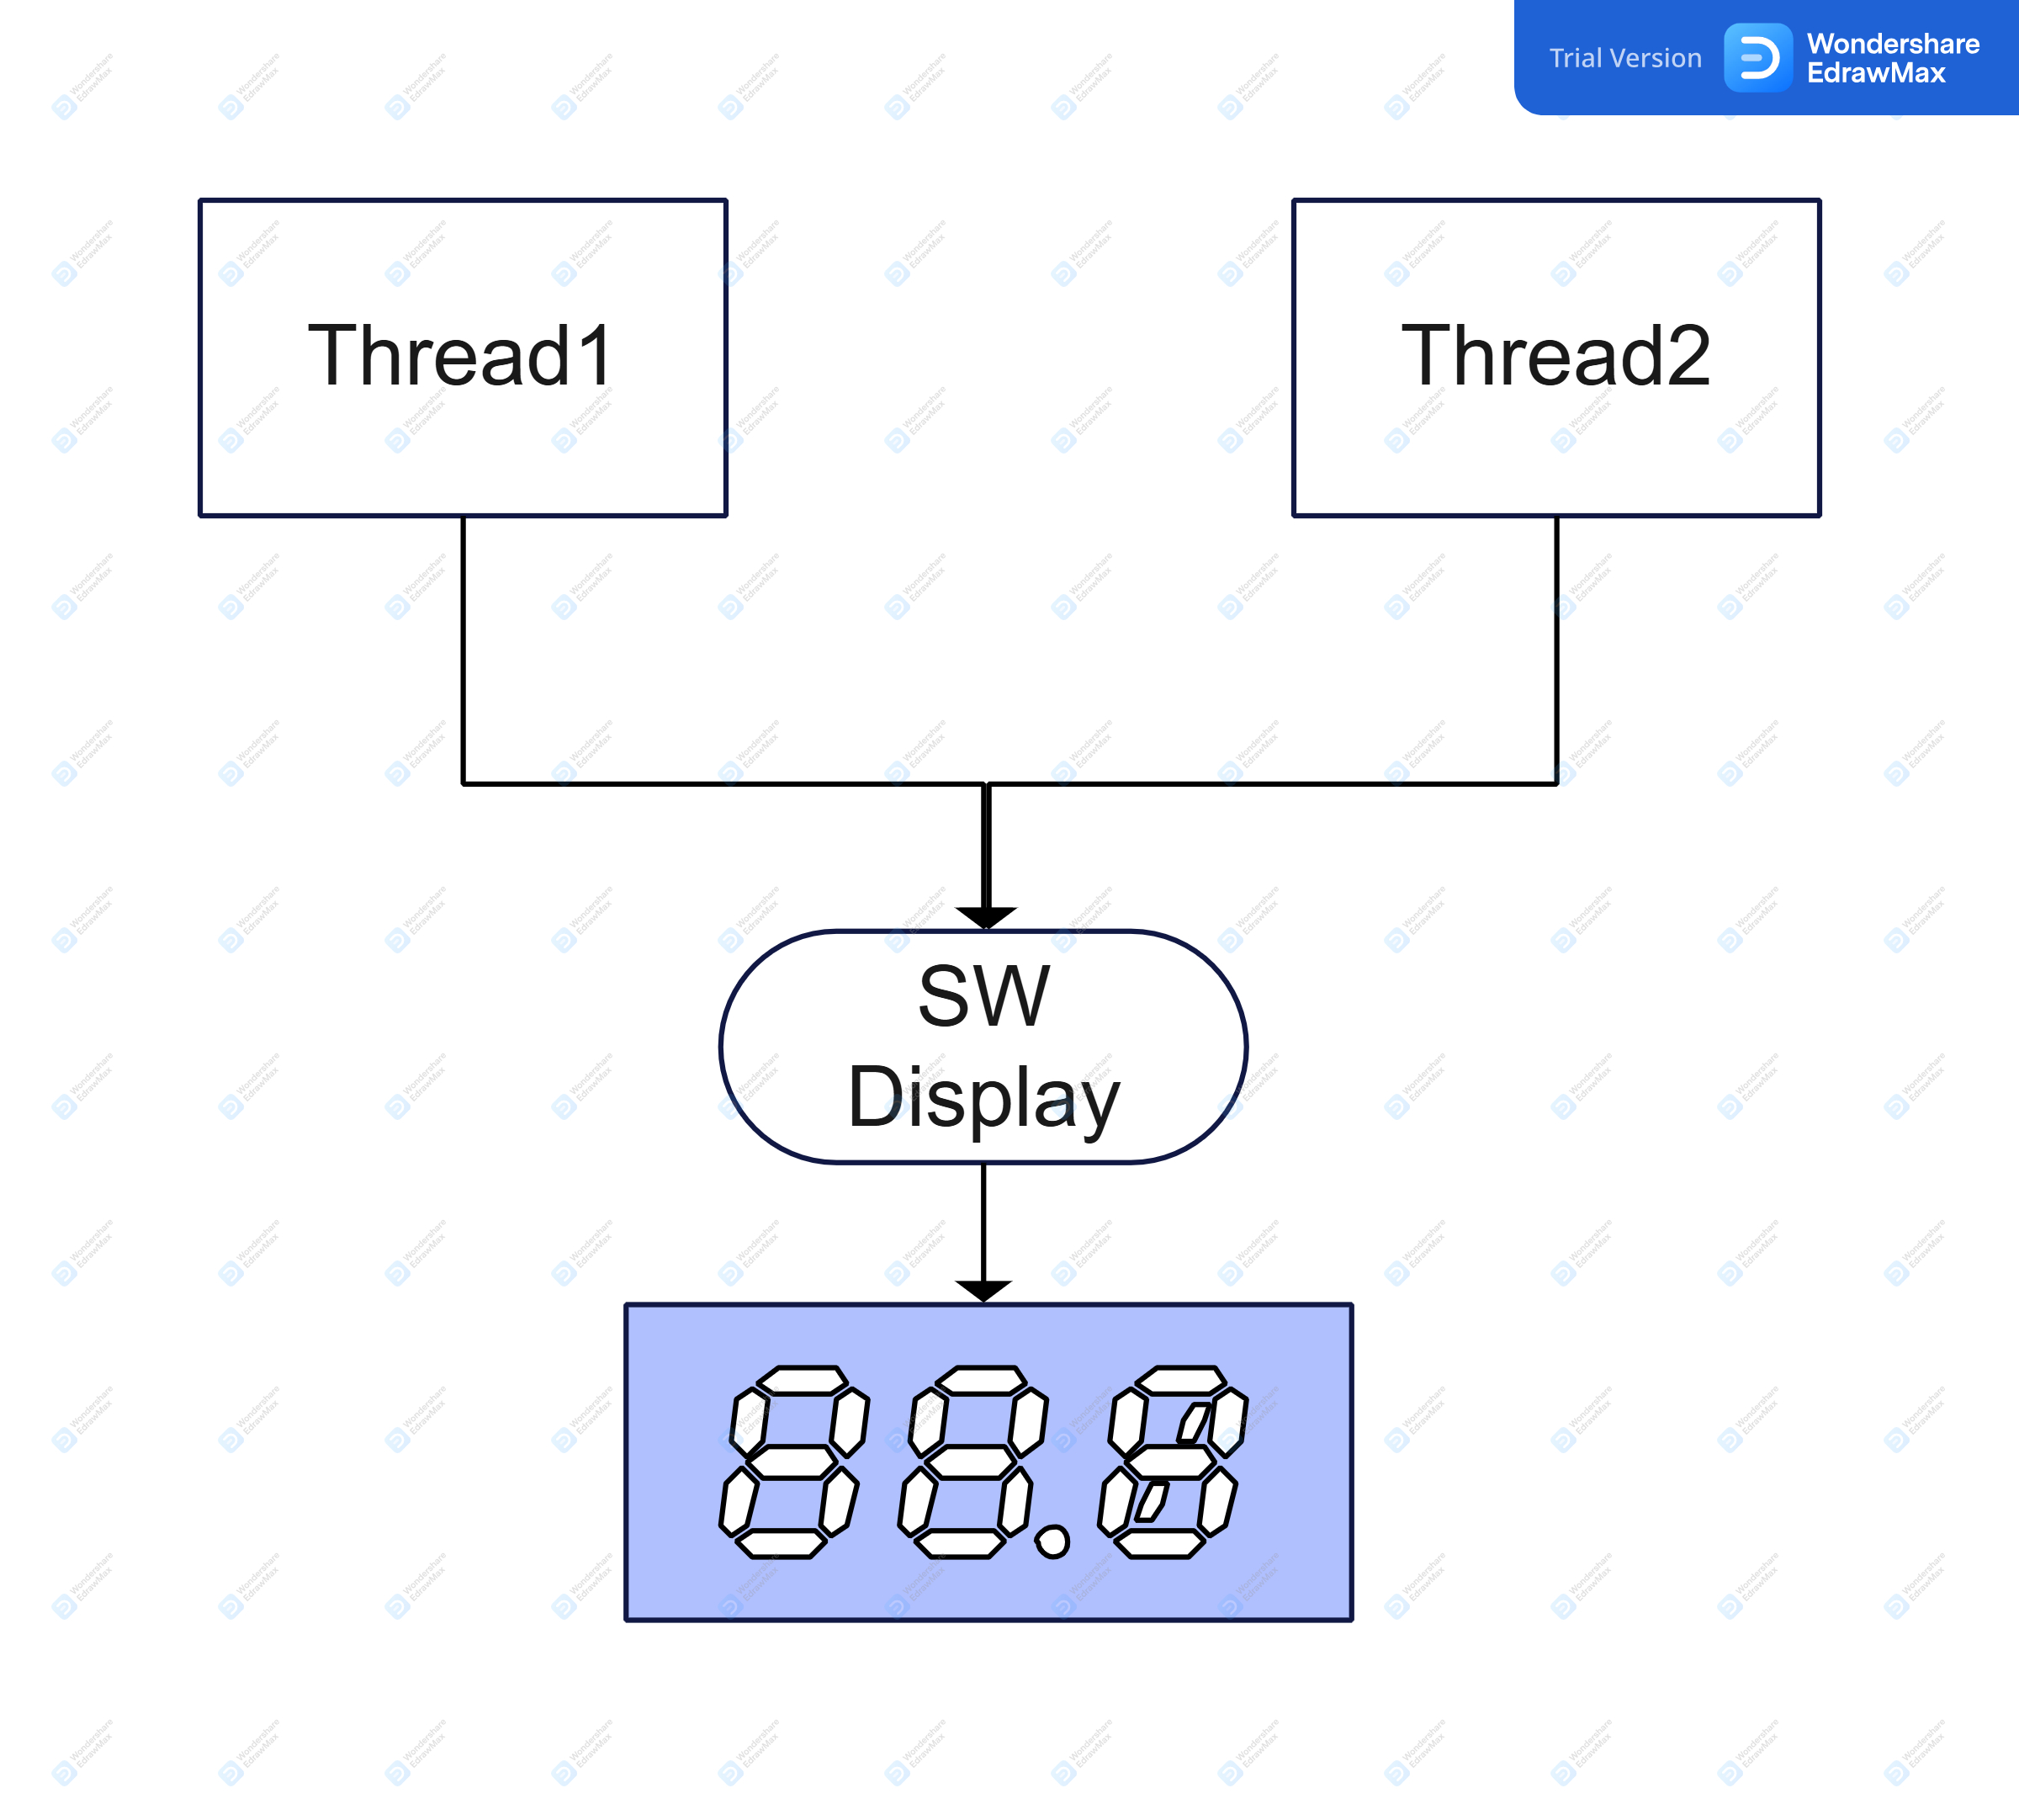
\includegraphics[scale=0.05]{presentation/threads.jpg}
        \end{column}
    \end{columns}
\end{frame}
\begin{frame}{CMSIS RTOs Sincronización}
    \begin{columns}
        \begin{column}{0.50\textwidth}
            \begin{itemize}
                \item Una posible solución. Se añade una cola gestionada por el Sistema Operativo
                \item Existe un thread que lee los mensajes que llegan a a la cola para enviarlos al display 
                \item Cada thread que quiere enviar un mensaje al LCD escribe en la cola
            \end{itemize}    
        \end{column}
        \begin{column}{0.50\textwidth}
            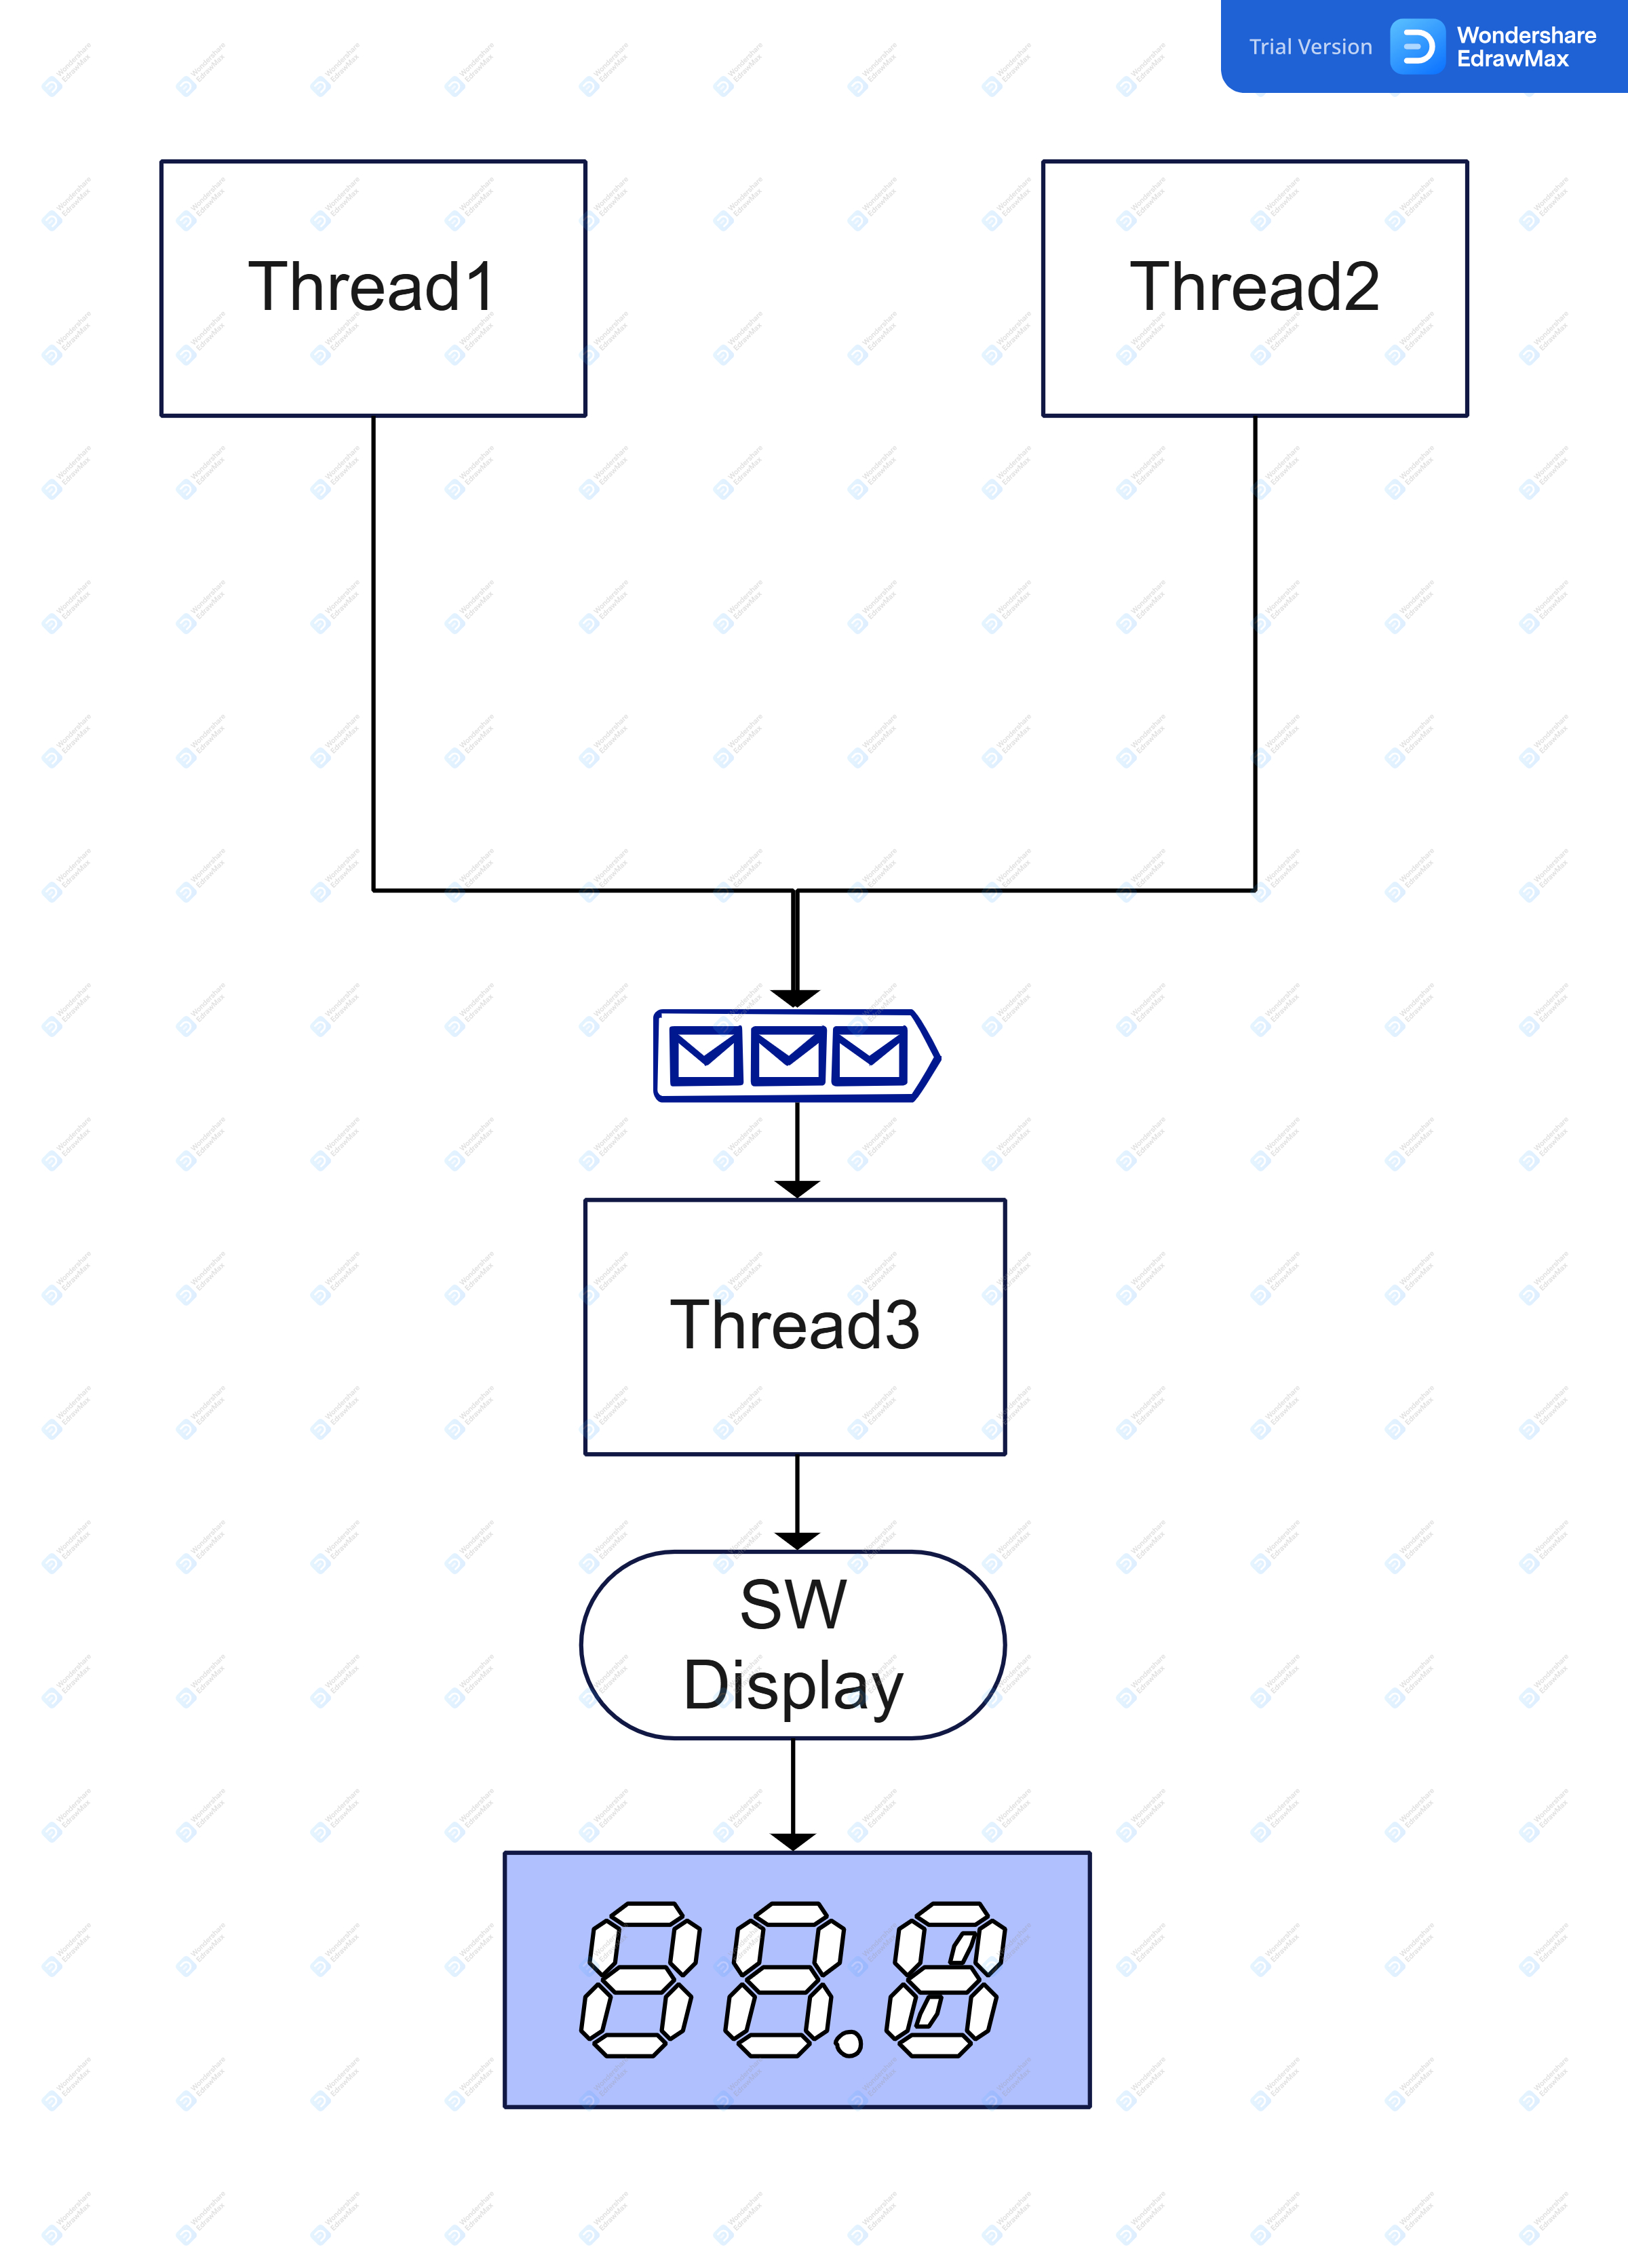
\includegraphics[scale=0.05]{presentation/threads-sync.jpg}
        \end{column}
    \end{columns}
\end{frame}

\begin{frame}[fragile]{Sincronización con Thread Flags}
      \begin{itemize}
          \item \textbf{Problema:} La tarea 1 genera periódicamente eventos/datos (1s). Queremos que la tarea 2 solo se ejecute cuando haya un dato disponible y que no consuma CPU mientras tanto.
      \end{itemize}
      \begin{columns}
            \begin{column}{0.50\textwidth}
                \begin{itemize}
                    \item[]                      
                    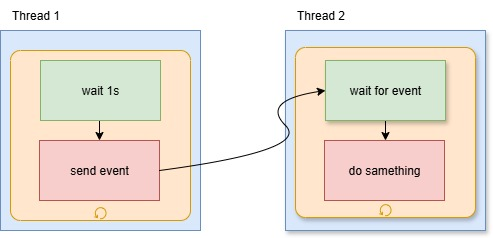
\includegraphics[scale=0.25]{presentation/flags.jpg}
                    \item El Thread 2 pasa al estado de \textbf{Waiting} hasta que el Thread 1 active el flag.
                    \item Cuando el flag o el conjunto de flags son activados el hilo pasa al estaddo \textbf{Ready}
                \end{itemize}
            \end{column}
            \begin{column}{0.50\textwidth}
             \begin{minted}[fontsize=\scriptsize, bgcolor=blue!5]{c}
void Thread1 (void *argument){
    while(1){
    osdelay(1000);
    osThreadFlagSet(tid_thread2, 0x0001);
    }
}

void Thread2 (void *argument){
    while(1){
    status = osThreadFlagWait(0x0001,
             osFlagsWaitAny, 
             osWaitForever);
    //
    }
}
             \end{minted}
             
            \end{column}
     \end{columns}
\end{frame}

\begin{frame}[fragile]{CMSIS RTOs Thead Flags}

    \begin{itemize}
        \item []
         \begin{minted}[fontsize=\scriptsize, bgcolor=blue!5]{c}
uint32_t osThreadFlagSet(osThreadId_t thread_id, uint32_t flags)
/* Activa el flag especificado de una tarea activa
Se puede llamar desde una interrupción */

         \end{minted}
         \begin{minted}[fontsize=\scriptsize, bgcolor=blue!5]{c}
uint32_t osThreadFlagClear(osThreadId_t thread_id, uint32_t signals)
/* Borra el flag especificado de una tarea activa
No se puede llamar desde una interrupción*/

         \end{minted}
         \begin{minted}[fontsize=\scriptsize, bgcolor=blue!5]{c}
uint32_t osThreadFlagsWait(uint32_t flags, uint32_t options, uint32_t timeout)
/* Espera a uno o más Flags para continuar la ejecución
No se puede llamar desde una interrupción */

         \end{minted}
         \begin{minted}[fontsize=\scriptsize, bgcolor=blue!5]{c}
uint32_t osThreadFlagGet(void)
/* Retorna los flags del thread en ejecución 
No se puede llamar desde una interrupción */

         \end{minted}      
         \item[] \href{https://arm-software.github.io/CMSIS_5/RTOS2/html/group__CMSIS__RTOS__ThreadFlagsMgmt.html}{CMSIS RTOS V2 Thread Flags reference}
    \end{itemize}     
\end{frame}

\begin{frame}[fragile]{CMSIS RTOS Colas}
\begin{itemize}
    \item Concepto de Productor/Consumidor. Un Thread o una ISR producen datos y un thread los consume
\end{itemize}
\begin{columns}
  \begin{column}{0.45\textwidth}     
    \begin{minted}[fontsize=\tiny, bgcolor=blue!5]{c}
int Init_Thread (void) {
  id_MsgQueue = osMessageQueueNew(16, 
                sizeof(uint8_t), NULL);
  tid_Thread = osThreadNew(Producer, NULL, NULL);
  if (tid_Thread == NULL) {   return(-1);  }
  tid_Thread = osThreadNew(Consumer, NULL, NULL);
  if (tid_Thread == NULL) {   return(-1);  }
  return(0);
}
void Producer (void *argument) {
    uint8_t index=0;
    osStatus_t status;
        while (1) {
        status=osMessageQueuePut(id_MsgQueue, 
                             &index, 0U, 0U);
        	index++;
        	osDelay(100);
        }
}
void Consumer (void *argument) {
while (1) {
	status = osMessageQueueGet(id_MsgQueue, 
               &val, NULL, osWatiForever );
  }
}

    \end{minted}
    \end{column}
    \begin{column}{0.55\textwidth}
     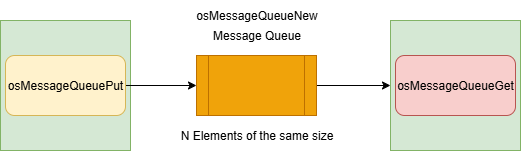
\includegraphics[scale=0.35]{presentation/queues.drawio.png}
    \end{column}
\end{columns}
\end{frame}

\begin{frame}[fragile]{CMSIS RTOs Colas}
    \begin{itemize}
        \item []
         \begin{minted}[fontsize=\scriptsize, bgcolor=blue!5]{c}
osMessageQueueId_t 	osMessageQueueNew (uint32_t msg_count, uint32_t msg_size, const osMessageQueueAttr_t *attr)
/* Create and Initialize a Message Queue object */
         \end{minted}
         \begin{minted}[fontsize=\scriptsize, bgcolor=blue!5]{c}
const char * 	osMessageQueueGetName (osMessageQueueId_t mq_id)
/* Get name of a Message Queue object. */
         \end{minted}
         \begin{minted}[fontsize=\scriptsize, bgcolor=blue!5]{c}
osStatus_t 	osMessageQueuePut (osMessageQueueId_t mq_id, const void *msg_ptr, uint8_t msg_prio, uint32_t timeout)
/* Put a Message into a Queue or timeout if Queue is full */
         \end{minted}
         \begin{minted}[fontsize=\scriptsize, bgcolor=blue!5]{c}
osStatus_t 	osMessageQueueGet (osMessageQueueId_t mq_id, void *msg_ptr, uint8_t *msg_prio, uint32_t timeout)
/* Get a Message from a Queue or timeout if Queue is empty */
         \end{minted}   
         \begin{minted}[fontsize=\scriptsize, bgcolor=blue!5]{c}
uint32_t 	osMessageQueueGetCapacity (osMessageQueueId_t mq_id)
/* Get maximum number of messages in a Message Queue */
         \end{minted}            
         \begin{minted}[fontsize=\scriptsize, bgcolor=blue!5]{c}
uint32_t 	osMessageQueueGetMsgSize (osMessageQueueId_t mq_id)
/* Get maximum message size in a Message Queue */
         \end{minted}
         \begin{minted}[fontsize=\scriptsize, bgcolor=blue!5]{c}
uint32_t 	osMessageQueueGetCount (osMessageQueueId_t mq_id)
/* 	Get number of queued messages in a Message Queue */
         \end{minted}
         \begin{minted}[fontsize=\scriptsize, bgcolor=blue!5]{c}
uint32_t 	osMessageQueueGetSpace (osMessageQueueId_t mq_id)
/* Get number of available slots for messages in a Message Queue */
         \end{minted}
         \begin{minted}[fontsize=\scriptsize, bgcolor=blue!5]{c}
osStatus_t 	osMessageQueueReset (osMessageQueueId_t mq_id)
/* Reset a Message Queue to initial empty state */
         \end{minted}
         \begin{minted}[fontsize=\scriptsize, bgcolor=blue!5]{c}
osStatus_t 	osMessageQueueDelete (osMessageQueueId_t mq_id)
/* 	Delete a Message Queue object */
         \end{minted}
                  
         \item[] \href{https://arm-software.github.io/CMSIS_5/RTOS2/html/group__CMSIS__RTOS__Message.html}{CMSIS RTOS V2 Thread Message Queue reference}
    \end{itemize}     
\end{frame}


\begin{frame}[fragile]{CMSIS Retardos y acciones temporizadas por \textbf{software}}
\begin{itemize}
    \item Funciones genéricas de espera Basadas en el SysTick Timer
    \begin{minted}[fontsize=\scriptsize, bgcolor=blue!5]{c}
osStatus_t status;
uint32_t delayTime=1000;
status = osdelay(delayTime); // tarea que se bloquea hasta que cumpla el tiempo
uint32_t tick;

tick = oskernelGetTickCount(); //obtiene el valor actual del system tick
for (;;){
    tick += 1000u;
    osdelayUnyil(tick); // Espera hasta que pasen 1000 ticks
}   
    \end{minted}
    \item \textbf{Estas funciones no se puede usar desde rutinas de atención a la interrupción}
    \item Timers virtuales
        \begin{itemize}
            \item Ejecutan una función (\textbf{csllback}) cuando el tiempo expira
            \item la función de callback es definida por el usuario
        \end{itemize}
\end{itemize}
    
\end{frame}

\begin{frame}[fragile]{CMSIS-RTOS Timer Virtuales}
    \begin{columns}
        \begin{column}{0.55\textwidth}    
        \begin{itemize}
        \item Los timers virtuales tienen dos modos de funcionamiento:
        \begin{itemize}
            \item \textbf{one-shot} Se arranca el timer y trancurrido un tiempo (configurable en pasos de Ticks) se ejecuta una callback, 
            \item \textbf{periodic} Se arranca el timer y cada vez que pasa el tiempo configurado se ejecuta la callback
            \item Estos timer virtuales no se pueden (ni deben) configurarse para ejecutarse con tiempo por debajo del ms
        \end{itemize}
        \end{itemize}
        \end{column}
        \begin{column} {0.45\textwidth} 
        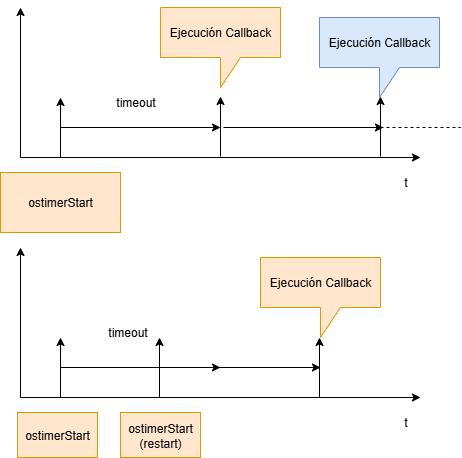
\includegraphics[scale=0.25]{presentation/softwaretimers.drawio.png}
     \end{column}
    \end{columns} 
\end{frame}

\begin{frame}[fragile]{CMSIS-RTOS Timer Virtuales}
    \begin{columns}
        \begin{column}{0.65\textwidth}
            \begin{minted}[fontsize=\scriptsize, bgcolor=blue!5]{c}
osTimerId_t swtim_id;
static uint32_t param=0;
/* Función de callback para el timer */
void TimerLed_Callback (void const *arg){
    LED_Toggle(LED1);
}

/* Inicialización del timer y arranque */
int Init_SWTImer (void){
    osStatus_t status;
    Init_LED(LED1);
    param=3;
    swtim_id = osTimerNew((osTimerFunc_t)&TimerLed_Callback, 
                          osTimerPeriodic, &param, NULL);
    if (swtim_id != NULL){
        status = osTimerStart(swtim_id, 1000U);
        if (status != osOk){
            return -1;
        }
    }
return 0;
}

        \end{minted}
     \end{column}
     \begin{column}{0.35\textwidth}
         \begin{itemize}
             \item El identificador del timer es usado por la función que lo arranca
             \item el timer se puede configurar como osTimerPeriodic u osTimerOnce
         \end{itemize}
     \end{column}
    \end{columns}
\end{frame}


\begin{frame}[fragile]{CMSIS RTOs Timers Software}
    \begin{itemize}
        \item Estas funciones \textbf{no se pueden llamar desde rutinas de interrupción}
        \item[]
        \item[] 
         \begin{minted}[fontsize=\scriptsize, bgcolor=blue!5]{c}
osTimerId_t 	osTimerNew (osTimerFunc_t func, osTimerType_t type, void *argument, const osTimerAttr_t *attr)
/+ Create and Initialize a timer. */
         \end{minted}
         \begin{minted}[fontsize=\scriptsize, bgcolor=blue!5]{c}
const char * 	osTimerGetName (osTimerId_t timer_id)
/* Get name of a timer. */
         \end{minted}
         \begin{minted}[fontsize=\scriptsize, bgcolor=blue!5]{c}
osStatus_t 	osTimerStart (osTimerId_t timer_id, uint32_t ticks)
/* Start or restart a timer. */
         \end{minted}
         \begin{minted}[fontsize=\scriptsize, bgcolor=blue!5]{c}
osStatus_t 	osTimerStop (osTimerId_t timer_id)
/* Stop a timer */
         \end{minted}   
         \begin{minted}[fontsize=\scriptsize, bgcolor=blue!5]{c}
uint32_t 	osTimerIsRunning (osTimerId_t timer_id)
/* Check if a timer is running. */
         \end{minted}            
         \begin{minted}[fontsize=\scriptsize, bgcolor=blue!5]{c}
osStatus_t 	osTimerDelete (osTimerId_t timer_id)
/* Delete a timer. */
         \end{minted}
                 
         \item[] \href{https://arm-software.github.io/CMSIS_5/RTOS2/html/group__CMSIS__RTOS__TimerMgmt.html}{CMSIS RTOS V2 Thread Message Queue reference}
    \end{itemize}     
\end{frame}
\section{Configuración y otras herramientas}
\begin{frame}{Estructura de los proyectos que usan CMSIS-RTOS}
\resizebox{0.9\textwidth}{!}{
\begin{forest}
for tree={
    grow'=south,
    draw,
    rectangle,
    node options={align=center, font=\Huge\ttfamily, inner sep=14pt},
    edge path={
        \noexpand\path [draw, \forestoption{edge}] (!u.parent anchor) --  (.child anchor)\forestoption{edge label};
    },
}
[Proyecto
  [Source Group 1
    [main.c]
    [utils.c]
    [More files]
  ]
  [\textcolor{red}{CMSIS}
    [rtx\_lib.c]
    [RTX\_Config.c]
    [\textcolor{green}{RTX\_Config.h}]
    [More files]
  ]
  [Device
    [stm32f4xx\_hal.c]
    [More files]
  ]
]
\end{forest}}
\begin{itemize}
    \item La figura solo muestra algunos ficheros 
    \item El fichero \textcolor{green}{RTX\_Config.h} permite configurar los parámetros del SO
\end{itemize}
\end{frame}

\begin{frame}{CMSIS-RTOS Configuración de parámetros}

\begin{table}[H]
\centering
\begin{tabular}{|l|l|}
\hline
\multicolumn{2}{|c|}{\textbf{Configuración del Sistema}} \\
\hline
Global Dynamic Memory Size & Tamaño de la memoria\\
kernel Tick Frequency & Frecuencia del tick sistema (Hz) \\
Round-Robin Thread Switching & Activar Round-Robin \\
Round-Robin Timeout & Tiempo de cambio de hilo \\
ISR FIFO QUEUE & Tamaño de cola FIFO para ISR \\
\hline
\multicolumn{2}{|c|}{\textbf{Configuración de Hilos}} \\
\hline
Default Thread Stack Size & Tamaño por defecto de pila de hilo \\
IDLE THREAD STACK SIZE & Pila del hilo idle \\
\hline
\multicolumn{2}{|c|}{\textbf{Timers}} \\
\hline
Timer Thread Priority & Prioridad del thread para los timers virtuales \\
Tamaño del stack & Pila del hilo de temporizador \\
OS\_TIMER\_THREAD\_TCB\_SIZE & TCB del hilo de temporizador \\
\hline
\end{tabular}
\caption{Algunos de los parámetros configurables en RTX\_Config.h agrupados por categoría}
\end{table}

    
\end{frame}

\begin{frame}{Watch Window RTX}
    \begin{itemize}
        \item Permite visualizar los objetos del sistema operativo RTX creados con CMSIS-RTOS
        \begin{columns}
            \begin{column}{0.50\textwidth}
            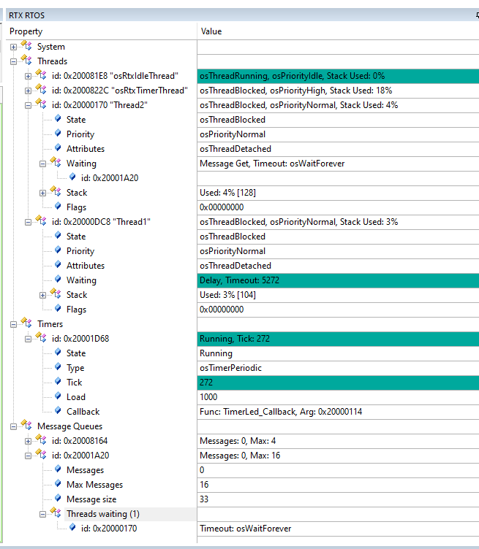
\includegraphics[scale=0.5]{presentation/watchwindowRTX.png}
                
            \end{column}
            \begin{column}{0.50\textwidth}
            \begin{itemize}
                \item osRtxidleThread Tarea idle del SO
                \item osRtxTimerThread Thread que gestiona los timers virtuales
                \item Thread1, Thread2, Threads creados en la aplicación
                \item Timers. id: 0x20001D68 Ejemplo de un timer periódico con sus detalles
                \item Message Queues. id: 0x20008164. Ejemplo de cola con tamaño 4. id: 0x20001A20. Cola de tamaño 16 mensajes. Cada mensaje ocupa 33 bytes. El thread con id:0x20000170 esta bloqueado esperando un mensaje en esta cola
                
            \end{itemize}
            \end{column}
        \end{columns}
    \end{itemize}
\end{frame}

\section{Consideraciones finales}
\begin{frame}{CMSIS-RTOS Consideraciones}
\begin{itemize}
    \item Antes de abordar una aplicación, se diseñará una estructura de la misma, de forma que en la medida de lo posible cada periférico será gestionado por un módulo software que estará compuesto por el correspondiente thread, señales, colas, y estructuras de datos. 
    \item Las ISRs serán manejadas por la HAL y en las respectivas Callbacks (poner atención a las Callbacks que se pueden definir con CMSIS-Driver para I2C/SPI y UART) se enviarán a los distintos threads las señales, mensajes necesarios. Serán rutinas cortas y se evitarán bucles. Vigilar que elementos del S.O. se pueden implementar en su interior.
    \item Prestar especial atención a la sincronización entre threads.
    |item Se reducirá al máximo la utilización de variables globales
\end{itemize}

\end{frame}
\begin{frame}{Ejercicios para comprender el uso de CMSIS RTOS V2}
    \begin{itemize}
        \item Disponibles in github \href{https://github.com/mruizlgz/SBM-rtos}{(sbm-rtos)}. Documentación en: \href{https://mruizglz.github.io/SBM-rtos}{(SPHINX DOC)} o \href{https://mruizglz.github.io/SBM-rtos/simplepdf/SBM-CMSIS-RTOS-V2.pdf}{(PDF)}
        
        \item Ejemplos:
            \begin{itemize}
                \item threads Creación de dos threads usando la misma función
                \item threads-flags Sincronización con flags
                \item threads-queues Sincronización con colas
                \item threads-timers Uso de timer virtuales
            \end{itemize}
    \end{itemize}
\end{frame}
